%\title{LaTeX Portrait Poster Template}
%%%%%%%%%%%%%%%%%%%%%%%%%%%%%%%%%%%%%%%%%
% a0poster Portrait Poster
% LaTeX Template
% Version 1.0 (22/06/13)
%
% The a0poster class was created by:
% Gerlinde Kettl and Matthias Weiser (tex@kettl.de)
% 
% Adapter by Jens Buysse for Hogeschool Gent
% This template has been downloaded from:
% http://www.LaTeXTemplates.com
%
% License:
% CC BY-NC-SA 3.0 (http://creativecommons.org/licenses/by-nc-sa/3.0/)
%
%%%%%%%%%%%%%%%%%%%%%%%%%%%%%%%%%%%%%%%%%

%----------------------------------------------------------------------------------------
%	PACKAGES AND OTHER DOCUMENT CONFIGURATIONS
%----------------------------------------------------------------------------------------

\documentclass[a0,portrait]{a0poster}

\usepackage{multicol} % This is so we can have multiple columns of text side-by-side
\columnsep=100pt % This is the amount of white space between the columns in the poster
\columnseprule=3pt % This is the thickness of the black line between the columns in the poster

\usepackage[svgnames]{xcolor} % Specify colors by their 'svgnames', for a full list of all colors available see here: http://www.latextemplates.com/svgnames-colors

\usepackage{times} % Use the times font
%\usepackage{palatino} % Uncomment to use the Palatino font

\usepackage{graphicx} % Required for including images
\graphicspath{{figures/}} % Location of the graphics files
\usepackage{booktabs} % Top and bottom rules for table
\usepackage[font=small,labelfont=bf]{caption} % Required for specifying captions to tables and figures
\usepackage{amsfonts, amsmath, amsthm, amssymb} % For math fonts, symbols and environments
\usepackage{wrapfig} % Allows wrapping text around tables and figures
\usepackage[export]{adjustbox}

\begin{document}
    
\hyphenpenalty 10000
\exhyphenpenalty 10000

%----------------------------------------------------------------------------------------
%	POSTER HEADER 
%----------------------------------------------------------------------------------------

% The header is divided into two boxes:
% The first is 75% wide and houses the title, subtitle, names, university/organization and contact information
% The second is 25% wide and houses a logo for your university/organization or a photo of you
% The widths of these boxes can be easily edited to accommodate your content as you see fit

\begin{minipage}[t]{0.75\linewidth}
\VeryHuge \color{HoGentAccent1} \textbf{Android zonder Google} \color{Black}\\ % Title
\Huge\textit{Waarom je Google zou willen vermijden in je Android smartphone en hoe je het kan doen}\\[2.4cm] % Subtitle
\huge \textbf{Verswijvelt Casper, Desmet Stein, Lewyllie Liesbeth}\\[0.5cm] % Author(s)
\huge Hogeschool Gent, Valentin Vaerwyckweg 1, 9000 Gent\\[0.4cm] % University/organization
\Large \texttt{casper.verswijvelt.y7500@student.hogent.be} \\
\end{minipage}
%
\begin{minipage}[t]{0.25\linewidth}

\includegraphics[width=13cm,right]{figures/HOGENT_Logo_Pos_rgb.png} 

\end{minipage}

\vspace{1cm} % A bit of extra whitespace between the header and poster content

%----------------------------------------------------------------------------------------

\begin{multicols}{2} % This is how many columns your poster will be broken into, a portrait poster is generally split into 2 columns

%----------------------------------------------------------------------------------------
%	ABSTRACT
%----------------------------------------------------------------------------------------

\color{HoGentAccent1} % Navy color for the abstract

\begin{abstract}
Binnen dit onderzoek werd er onderzocht welke methoden er precies zijn, al dan niet ondersteund door Google en/of Android, om Google zoveel mogelijk te verbannen van een Android apparaat, en hoe effectief ze juist zijn.
\end{abstract}
%----------------------------------------------------------------------------------------
%	INTRODUCTION
%----------------------------------------------------------------------------------------

\setlength{\parskip}{\baselineskip}%
\setlength{\parindent}{0pt}%

\color{HoGentAccent1} 
\section*{Introductie}
\color{black}
\color{black}
Android telt de dag van vandaag reeds meer dan 2,5 miljard maandelijks actieve gebruikers. Android zelf is een zeer brede term. Deze bevat niet enkel het Android Open Source Project (AOSP), die de basisversie van het besturingssysteem omvat, maar ook alle aftakkingen hiervan. Zo'n aftakkingen worden vaak uitgebreid met extra functionaliteiten waarmee smartphone producenten zich proberen te onderscheiden van elkaar. Een ander softwarepakket dat vaak wordt meegeleverd met apparaten die bestemd zijn voor de westerse markt, maar niet inbegrepen is in het AOSP, is het 'Google Apps' pakket.

Google Apps, is niet, zoals de naam impliceert, enkel een verwijzing naar Google applicaties zoals Gmail, YouTube, Maps, etc. Hieronder valt ook het onderliggende 'Google Play Services' framework. Dit framework biedt API's aan die makkelijker te gebruiken zijn dan degene die in het AOSP te vinden zijn, en ook meer functionaliteiten aanbieden. Het 'Google Apps' softwarepakket staat apart van het besturingssysteem, en kan ook geüpdatet worden zonder dat het volledige besturingssysteem moet worden bijgewerkt. Zo kunnen applicatie-ontwikkelaars zeer makkelijk verderwerken met de nieuwste functionaliteiten die de Google Play Services aanbiedt, zelfs op apparaten die niet de laatste versie van Android bevatten.

Wanneer applicaties uit dit softwarepakket worden gebruikt, wordt er ook data verzameld over de gebruiker. Deze data gebruikt Google dan om gericht advertenties te kunnen sturen naar gebruikers. Volgens een onderzoek door Douglas C. Schmidt is Android een essentiële factor bij Google's verzamelen van data. De producten die Google aanbiedt zijn in staat om gebruikersgegevens te verzamelen via een verscheidenheid aan technieken die door de doorsnee gebruiker mogelijk moeilijk te begrijpen zijn. Een groot deel van de verzamelde data wordt verzameld wanneer de gebruiker niet rechtstreeks in contact komt met Google's producten. 

Applicaties binnen dit softwarepakket worden, wanneer deze wordt meegeleverd met het besturingssysteem, geïnstalleerd als systeemapplicaties. Dit betekent dat ze nooit volledig verwijderd kunnen worden. Dit wordt een probleem wanneer de gebruiker wil beperken welke Google software er zich op zijn/haar apparaat bevindt. Google zelf biedt reeds enkele opties aan om het verzamelen van data in te perken, maar deze zijn beperkt.
%----------------------------------------------------------------------------------------
%	GEOLOGY
%----------------------------------------------------------------------------------------

\color{Black} % DarkSlateGray color for the rest of the content
\color{HoGentAccent1} 
\section*{Experimenten}
\color{black}
Er werd reeds onderzocht hoeveel een standaard ingesteld Android apparaat communiceert met Google, maar dit werd nog niet toegepast samen met verschillende 'ontgoogle' methodes. In dit onderzoek werd onderzocht wat de mogelijke manieren zijn om Google zoveel mogelijk te verbannen van het apparaat, beide door methoden die Google zelf aanbiedt en methoden die niet rechtstreeks door Google ondersteund worden. Hieruit kwamen drie testgevallen voort: 
\begin{itemize}
    \item Android met fabrieksinstellingen
    \item Android met aangepaste instellingen 
    \item Aangepaste versie van Android. (LineageOS)
\end{itemize}

Bij elk testgeval werd bekeken welke stappen moesten worden gevolgd om de gewenste toestand van het testgeval te bereiken. Hierna werd er per geval geanalyseerd hoeveel keer er naar Google gecommuniceerd werd, zonder dat er enige interactie met het apparaat plaatsvond. 

\vfill\null
\columnbreak

\color{HoGentAccent1} 
\section*{Resultaten}
\color{black}


\begin{center}\vspace{1cm}
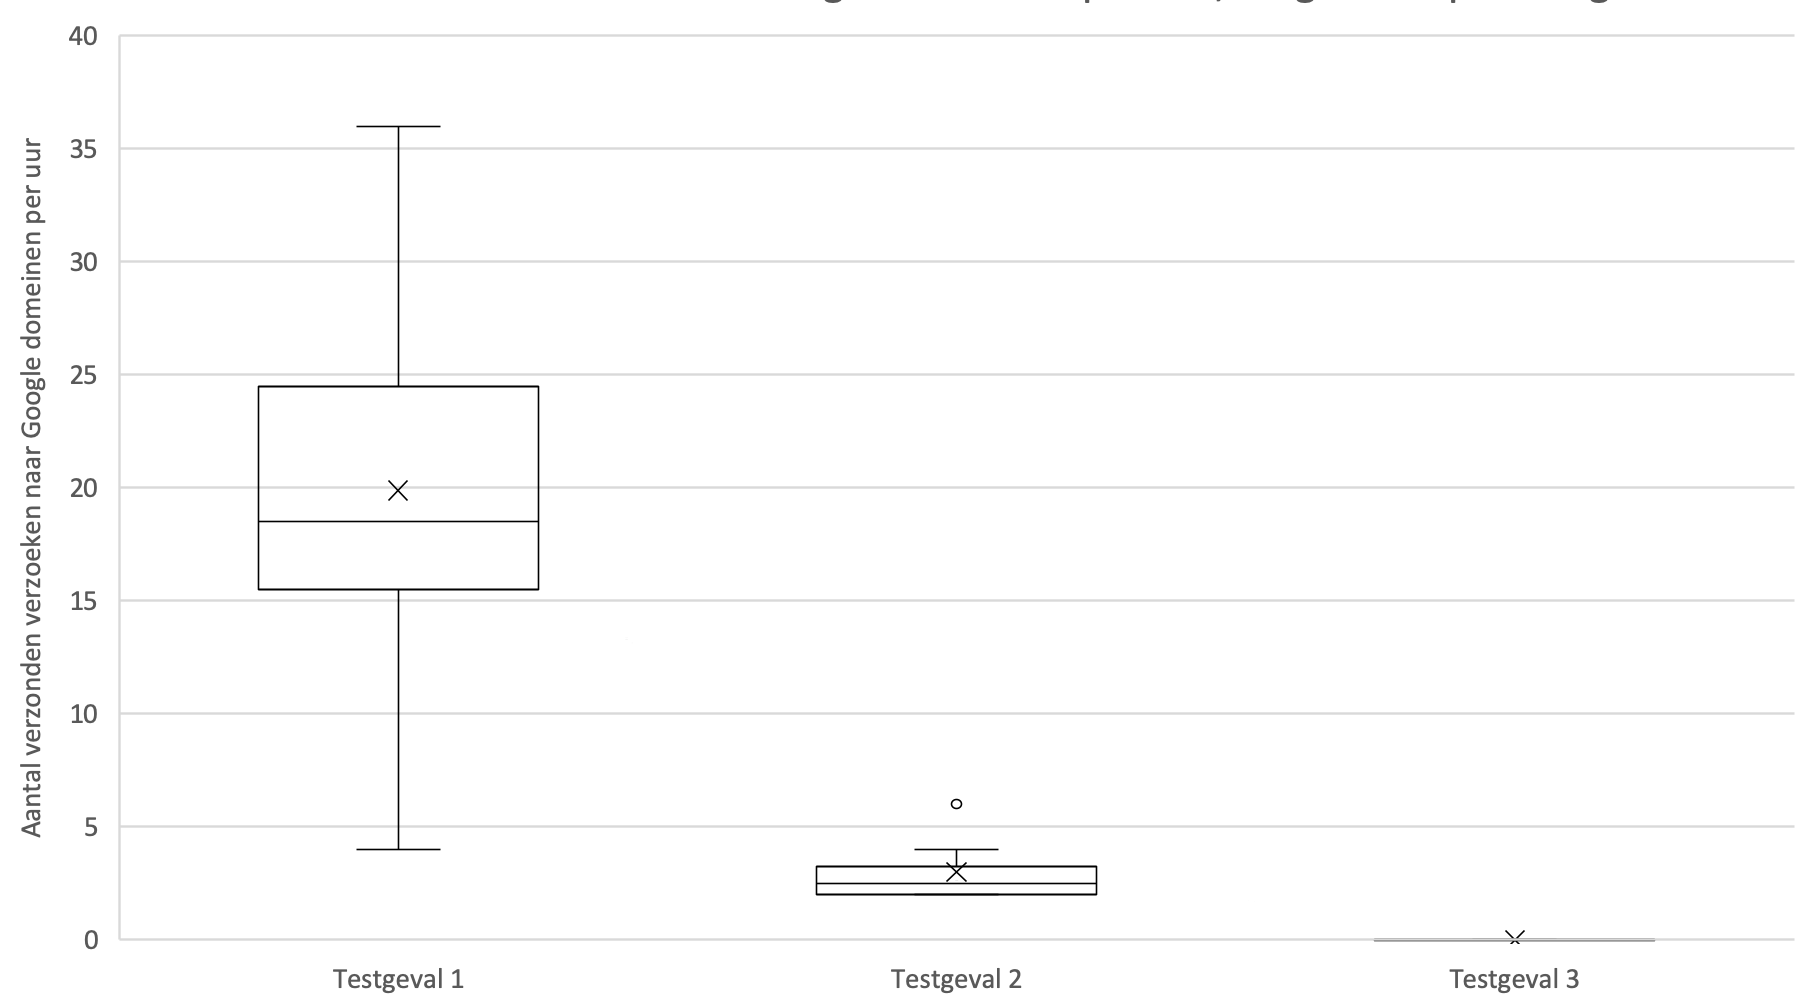
\includegraphics[width=1.0\linewidth]{../bachproef/experiment/grafieken/boxplot-compare-wide.png}
\captionof{figure}{\color{HoGentAccent5} Aantal verzonden verzoeken naar Google domeinen per uur, vergeleken per testgeval}
\label{grafiek}
\end{center}\vspace{1cm}

%------------------------------------------------

\color{HoGentAccent1} 
\section*{Conclusies}
\color{black}
Uit de resultaten van dit experiment bleek dat er per uur gemiddeld 20 keer naar Google werd gecommuniceerd wanneer het Android apparaat is ingesteld volgens de standaard instellingen. Het aantal verzonden verzoeken in deze toestand was zeer uiteenlopend wanneer dit werd vergeleken met de resultaten van het experiment bij de andere testgevallen. Dit aantal lag hier minimum op 4 verzoeken per uur en maximum op 36.

In het geval waar Google zoveel mogelijk werd ingetoomd door de opties aangeboden door Google en Android te gebruiken, werd er gemiddeld 3 keer per uur naar Google toe gecommuniceerd. Dit aantal ligt direct een stuk lager dan bij het voorgaande experiment, en met een minimum van 2 verzoeken en een maximum van 6 verzoeken zijn deze resultaten ook veel minder uiteenlopend. Tegenover het voorgaande testgeval werd het aantal verzoeken met 85\% gereduceerd. De stappen die moesten worden gevolgd om dit resultaat te bekomen, waren niet direct intuïtief te vinden binnen het Android besturingssysteem, maar eens gevonden zijn ze makkelijk aan te passen.

In het laatste geval werd er op het testapparaat een andere versie van Android geïnstalleerd, die geen enkele extra software van Google bevat, namelijk LineageOS. De stappen die hiervoor moesten gevolgd worden, waren alles behalve gebruiksvriendelijk. De benodigdheid van extra software die niet op een centrale plek op het internet wordt aangeboden is mogelijk een struikelblok voor gebruikers indien ze deze methode zelf ook willen toepassen. De stappen moeten zeer specifiek opgevolgd worden en de mogelijkheid dat het apparaat in een onbruikbare staat terechtkomt, is reëel. De moeite wordt wel beloond, want uit de resultaten blijkt dat er doorheen alle uitvoeringen van het experiment geen enkele communicatie met Google voorkomt in deze toestand.

In figuur \ref{grafiek} is te zien hoeveel communicaties naar Google er per uur plaatsvinden, vergeleken onder de verschillende testgevallen.
%----------------------------------------------------------------------------------------
%	FORTHCOMING RESEARCH
%----------------------------------------------------------------------------------------
\color{HoGentAccent1}
\section*{Toekomstig onderzoek}
\color{black}

Binnen dit onderzoek werd de inhoud en specifieke URL van aanvragen naar Google niet geanalyseerd. De inhoud van deze aanvragen kan echter wel meer licht laten schijnen op welke informatie er precies wordt gecommuniceerd naar Google toe. Verder kan het ook interessant zijn dit experiment toe te passen op een 'day-in-the-life' scenario om zo een meer realistische werklast op het apparaat uit te oefenen.


%----------------------------------------------------------------------------------------

\end{multicols}
\end{document}